% !TEX TS-program = pdflatex
% !TEX encoding = UTF-8 Unicode

% This is a simple template for a LaTeX document using the "article" class.
% See "book", "report", "letter" for other types of document.

\documentclass[12pt]{article} % use larger type; default would be 10pt

\usepackage[utf8]{inputenc} % set input encoding (not needed with XeLaTeX)

%%% Examples of Article customizations
% These packages are optional, depending whether you want the features they provide.
% See the LaTeX Companion or other references for full information.

%%% PAGE DIMENSIONS
\usepackage[a4paper,left=2cm,right=2cm,top=2cm,bottom=2cm]{geometry}
%\usepackage{geometry} % to change the page dimensions
% \geometry{a4paper} % or letterpaper (US) or a5paper or....
% \geometry{margin=0in} % for example, change the margins to 2 inches all round
% \geometry{landscape} % set up the page for landscape
%   read geometry.pdf for detailed page layout information

\usepackage{graphicx} % support the \includegraphics command and options

\usepackage[parfill]{parskip} % Activate to begin paragraphs with an empty line rather than an indent

%%% PACKAGES
\usepackage{booktabs} % for much better looking tables
\usepackage{array} % for better arrays (eg matrices) in maths
\usepackage{paralist} % very flexible & customisable lists (eg. enumerate/itemize, etc.)
\usepackage{verbatim} % adds environment for commenting out blocks of text & for better verbatim
\usepackage{subfig} % make it possible to include more than one captioned figure/table in a single float
\usepackage{amsmath}
\usepackage{amssymb}
\usepackage{logicproof}
\usepackage{tikz}
\usepackage{hyperref}
\usetikzlibrary{arrows,petri,topaths}
\usepackage{float}
\usepackage{graphicx}
\usepackage[T1]{fontenc}
\usepackage{listings}
\usepackage{pdflscape}
\lstset{
  basicstyle=\ttfamily,
  mathescape
}	
% These packages are all incorporated in the memoir class to one degree or another...

%%% HEADERS & FOOTERS
\usepackage{fancyhdr} % This should be set AFTER setting up the page geometry
\pagestyle{fancy} % options: empty , plain , fancy
\renewcommand{\headrulewidth}{0pt} % customise the layout...
\lhead{}\chead{}\rhead{}
\lfoot{}\cfoot{\sffamily\thepage\normalfont}\rfoot{}

%%% SECTION TITLE APPEARANCE
\usepackage{sectsty}
\allsectionsfont{\sffamily\mdseries\upshape} % (See the fntguide.pdf for font help)
% (This matches ConTeXt defaults)

%%% ToC (table of contents) APPEARANCE
\usepackage[nottoc,notlof,notlot]{tocbibind} % Put the bibliography in the ToC
\usepackage[titles,subfigure]{tocloft} % Alter the style of the Table of Contents
\renewcommand{\cftsecfont}{\rmfamily\mdseries\upshape}
\renewcommand{\cftsecpagefont}{\rmfamily\mdseries\upshape} % No bold!
\newcommand{\qedsymbol}{\rightline{$\blacksquare$}}
\renewcommand{\familydefault}{\sfdefault}
%\renewcommand{\thesection}{\hspace{-0.5cm}\arabic{section}}
\renewcommand{\thesubsection}{\alph{subsection})}
\renewcommand{\thesubsubsection}{}

\usepackage[style=authoryear]{biblatex}
\addbibresource{library.bib}

%%% END Article customizations

%%% The "real" document content comes below...

\title{\vspace{-1.6cm}Computational Modelling in the Humanities and Social Sciences Assignment \\
	\vspace{0.5cm}\large Measuring city accessibility using OpenStreetMap data\vspace{-0.3cm}}
\author{zrlr73}
\date{} % Activate to display a given date or no date (if empty),
         % otherwise the current date is printed 

\begin{document}
\maketitle

\section{Introduction}

As an occasional OpenStreetMap (OSM) contributor, I decided that using data directly from OSM in my assignment would be interesting. When a friend told me about a problem she had read about in \textit{Invisible Women} by Caroline Criado Pérez (\cite{Perez2019}), I decided to try and produce a tool that is applicable to this issue.

The problem is that cities are designed by commuting men, and therefore can end up optimised for this subset of the population, to the detriment of others. The book specifically discusses women, who have different travel patterns to men due to their (usually) increased care responsibilities and different way of life.

For example, many cities feature a `radial' transit network: designed with links that lead from the suburbs into the city centre, with infrastructure for transferring between these transit lines in the centre. Unfortunately, this system often fails to serve those who do not commute into the city centre for their work on a daily basis. Those who, for example, only need to travel among the suburbs, find themselves facing unreasonable journey times.

Similarly, cities are often designed for cars. With many households owning one or no cars, and any car that does exist usually being allocated to a commuter, those who stay at home may struggle to travel - not helped by the fact that, thanks to space constraints, more developed roads often worsen the experience for pedestrians. Pavements may be partially blocked with street furniture such as street lights and parking machines, or otherwise too narrow for buggies or for people with shopping to pass each other comfortably. As it is usually women who perform errands such as taking children out of the house or going to the shops, they are the ones who bear most of the brunt of these poor design choices.

Clearly, I am unable to directly change these problems. However, I thought it would be interesting to attempt to create a tool that, given an OpenStreetMap file covering a city, will score that city on its accessibility to non-commuters, such as those with care responsibilities. Given that OSM is a Volunteered Geographic Information (VGI) project, this will be complicated by the fact that I cannot rely on the data to be accurate, current or even present (with the last being the most likely scenario for many cities). Therefore I will need to attempt to utilise metrics that are (relatively) unaffected by lack of correct data.

There is also no guarantee that the provided data will perfectly encompass a city - it may be that the exported data includes some areas of countryside, or does not include all of the suburbs. The `true' boundary of a city is often a hotly discussed topic. In general, this means I will need to make use of relative information (eg, ratio of feature $x$ against feature $y$) instead of absolute information (eg, density of feature $x$ per square kilometre).


\section{Tools Utilised}
For this project, I have employed a number of programmatic tools, listed below:

\subsection{Python 3.9.2}
I am performing all of the required processing and analysis in Python, as it is well-supported by the open-source community, is accessible and popular, and performs well. Version 3.9.2 was used as it was already installed on my computer and is only three patches behind the latest version.

\subsection{BBBike Download Server}
This web application, available at \href{https://download.bbbike.org/osm/}{https://download.bbbike.org/osm/}, allows users to download extracts of the OSM map. I employed this tool to extract custom data for a number of cities, predominantly within the UK. These files were all downloaded in Protocolbuffer Binary Format (PBF; \texttt{.osm.pbf}) file format.

\subsection{PyDriosm}
PyDriosm is an open-source library which provides features for the parsing and storage of OSM data. Its main use in my software is to parse downloaded PBF files with the \href{https://pydriosm.readthedocs.io/en/latest/_generated/pydriosm.reader.parse_osm_pbf.html}{\texttt{pydriosm.reader.parse\_osm\_pbf()}} function, returning the data as a Python \texttt{dict}. PyDriosm can be installed using \texttt{pip}, with the package name \texttt{pydriosm}.

When installing on Windows 10 / Python 3.9.2, I had some trouble building the \texttt{GDAL} dependency - resolving this required installing Visual C++ build tools from Microsoft and then manually installing \texttt{GDAL} itself using a wheel file. More information on this can be found in the \href{https://pydriosm.readthedocs.io/en/latest/installation.html}{PyDriosm documentation}.

\subsection{tqdm}
\href{https://tqdm.github.io/}{\texttt{tqdm}} is a lightweight Python module for adding progress bars to iterative processes. I have employed it here to monitor progress on analysis steps.

\subsection{Co-ordinate distance measurement}
Finally, I adapted some code from \href{https://stackoverflow.com/a/19412565}{StackOverflow} to compute the surface distance between two co-ordinates for my \texttt{findDistance()} function.


\section{Implementation}
One major issue that was encountered was the very large times required to load PBF files into usable Python structures. Therefore, I started by creating a wrapper function, \texttt{ParsePBF()}. This function, upon reading a new PBF file, stores the parsed structure to disk in a "\texttt{cache}" folder using Python's inbuilt \href{https://docs.python.org/3/library/pickle.html}{\texttt{pickle}} library. Upon being asked to load the same file again, it would then check for the existence of an existing cache file before attempting to load it from the PBF. Loading these pickle files takes on the order of seconds, whereas large PBF map dumps have taken up to an hour to parse in my experience (using an Intel Core i5-6300HQ).

Methods that I came up with to measure a city's accessibility are as follows:

\subsection{Transport network layout}
Firstly, I sought to address the problem of transit system design. My idea was to find the number of `routes' (eg, train lines, bus routes) that each station / stop was on, for every station / stop, and then find the standard deviation across the city. A large standard deviation would indicate the presence of both many highly-connected stations and many poorly-connected stations, which would be most likely caused by a radial structure with weakly-connected suburban transport links and a strongly-connected `downtown' area. Conversely, a low standard deviation would indicate even distribution of transport links across the city, and therefore increased accessibility for those that do not commute into the city to work.

Unfortunately, upon attempting to access this data, I found that the majority of stations simply are not tagged with any information on which route(s) they are on. Some examples of urban metro networks do store limited line information, but these are the exception rather than the norm. Indeed, from my limited testing of various cities, London was the only one which stored a list of lines with each station, and even that was only for Underground lines. Similarly, bus stops also are not tagged with the bus routes that stop there. Stations with no lines are modelled as only being on 1 line, but this is clearly not a particularly reliable assumption (for example, Clapham Junction, one of the busiest stations in London, is overground-only and therefore taken to only be on one line)!

I believe that the problem here is that OSM data is designed to provide information to be used to create a graphical map - and more nuanced data on how stations relate to one another is simply not required. Given more time, I would try to cross-reference railway line data with station co-ordinates, or use alternative data sources such as \href{https://www.openrailwaymap.org/}{OpenRailwayMap}, but this was unfortunately not feasible for this project's timeframe. For the time being, I have implemented it anyway, assuming stations with no tagged lines have only 1, but I also provide the percentage of stations with no tagged lines in order to allow the user to judge the reliability of the metric for themselves.

\subsection{Cycle share schemes}
I also had the idea of measuring the presence of bike share schemes (for example, London's \href{https://tfl.gov.uk/modes/cycling/santander-cycles}{Santander Cycles} system), but articles I found on these appear to report that their benefits for non-commuters are inconclusive because they are typically optimised for city-centre commuter use rather than more local suburban journeys \parencite{Beecham2014}. Since the level of benefit for non-commuters versus commuters is not agreed upon, I decided to omit processing them.

\subsection{Mixed-use planning}
One method with which I did have some success was attempting to measure the level of zoning. While areas of cities are traditionally allocated specific purposes (residential, retail, industrial etc), in a practice known as single-use zoning, \cite{Perez2019} points out that this method of planning hugely hinders those who don't have access to a car, or live in areas with poorer public transport links. Cities like Vienna have had more success with mixed-use zoning: the design of cities where all residential areas are constructed alongside amenities such as schools, bus stops playgrounds, doctors' surgeries and shops. This ensures that the majority of services can be found within walking distance of a house, and also increases the perceived safety of residential areas through improved lighting and increased night-time activity.

Therefore, I decided to measure the average distance from a house to the nearest instance of each of these services. In order to avoid exhaustively checking the distance to, for example, every school in the city, for each house, I came up with an idea: sorting the list of schools' co-ordinates, finding a school that's somewhat near the given house through sampling across the list and then limiting the search to only schools that have a longitude within that distance of the house's longitude. This worked well, reducing complexity by well over half in my observations.

\subsection{Transport optimisation}
Since cars are not ubiquitous, and the individuals being considered here may well not have access to a car, we can reasonably assume that cities with large quantities of car infrastructure (relative to public transport provision) will be less accessible for them.

Therefore, the final method I implemented was one to count the number of bus stops, tram stops, stations and parking spaces. These were then divided to find:

\begin{itemize}
	\item The number of parking spaces per bus / tram stop
	\item The number of parking spaces per train station
	\item The number of parking spaces divided by $\text{"n\_stations"}\times 20 + \text{"n\_busStops"} + \text{"n\_tramStops"}$
\end{itemize}

The last item essentially produces a single overall ratio, with a single train station being modelled to have the same `value' as 20 bus / tram stops. This allows values to be compared between cities that may have differing levels of development on their bus, tram and train networks.


\section{Evaluation}
Since this program evaluates statistics on different cities, probably the best way to evaluate it is by looking at the information it provides. During the course of development, I have accumulated a number of different map dumps of various sizes, and the results can be seen in figure \ref{Fig:1}.

\begin{figure}
	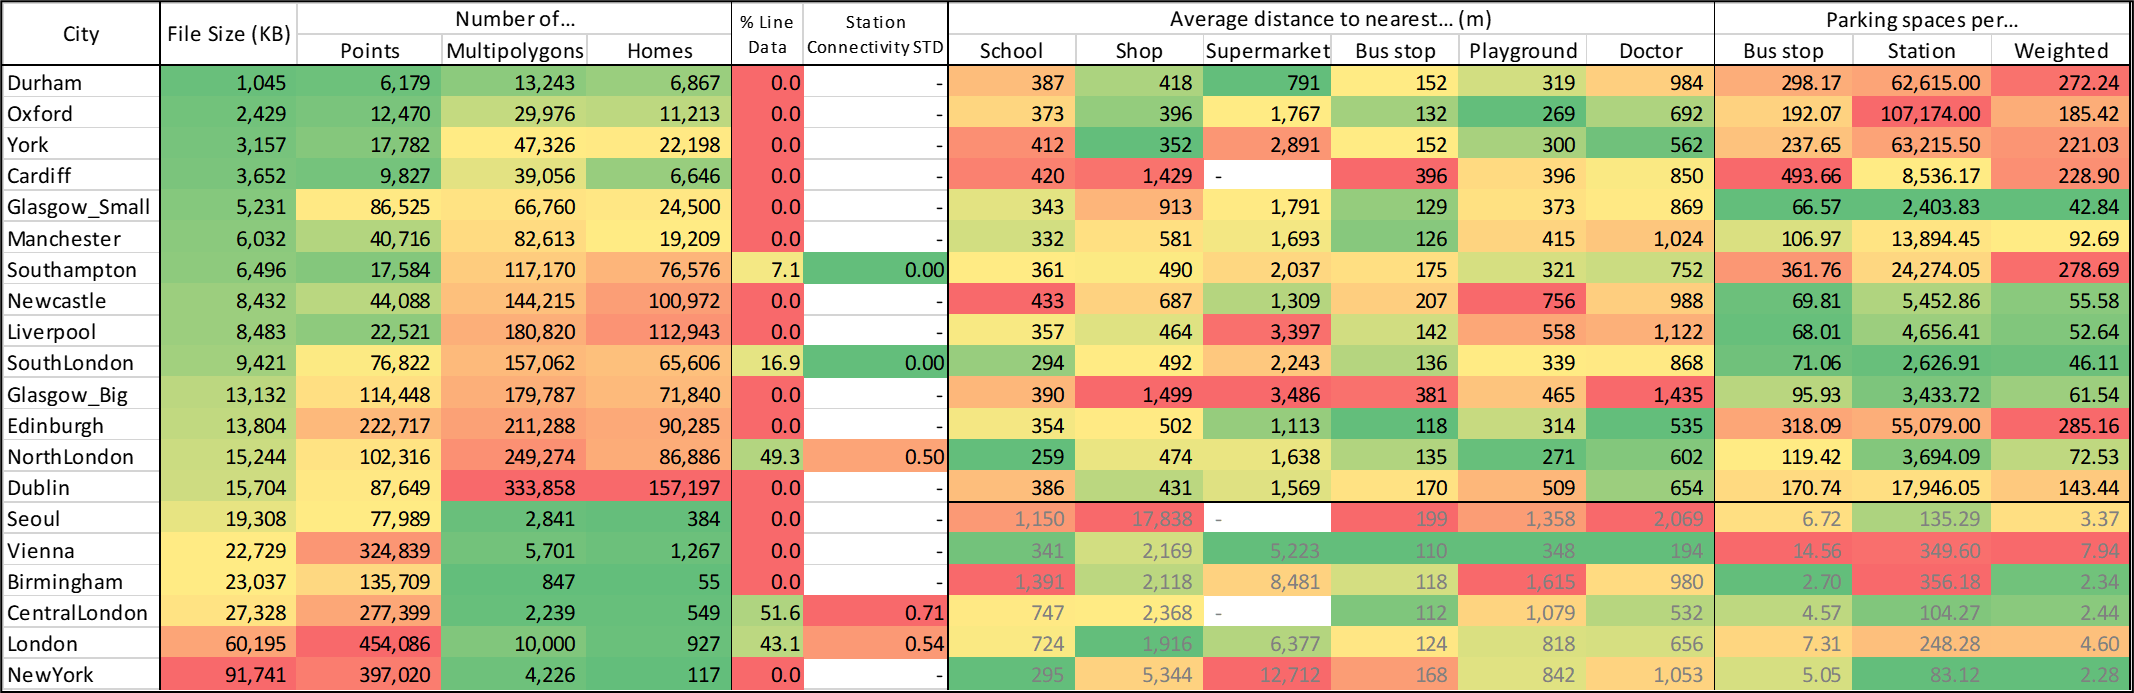
\includegraphics[width=\textwidth]{data.png}
	\caption{Data for a number of cities, ordered by file size ascending}
	\label{Fig:1}
\end{figure}

Unfortunately, there appears to be a bug in \texttt{PyDriosm} (which I use to import the city data), as any city over approximately 15MB seems to have a vastly reduced number of multipolygons (ie, features that represent an area on the map, rather than a point or a line). Also of note is that London appears to have exactly 10,000 multipolygons - which seems unlikely. This means that any feature that is stored as an area (including the majority of residential buildings and car parks) will be underrepresented, and therefore most data for cities larger than this size is invalid. To check this, I took subsets of the London export area (NorthLondon, SouthLondon and CentralLondon) and the former two, being smaller than the 15MB cutoff, appear to have been imported correctly (and have far more multipolygons than their superset!).

I am treating the data from these larger files as unreliable, and have included it for completeness but used separate conditional formatting rules to ensure that the top half still usefully covers the valid value range, and have also used grey text to indicate which data are problematic.

\subsection{Transport network layout}
I made the decision to include the station connectivity data because, while almost all city files yield no useful information, the results for the different areas of London are still interesting (and valid for larger cities, as stations are modelled as points rather than multipolygons). For reference purposes, the Tube map can be found \href{https://content.tfl.gov.uk/standard-tube-map.pdf}{here}, and a wider map including National Rail overground services \href{https://content.tfl.gov.uk/london-rail-and-tube-services-map.pdf}{here}.

The north side of London contains most of the `downtown' area, and therefore the majority of London Underground interchange stations (with up to 6 Tube lines per station in some cases such as King's Cross), as well as wider-reaching `spokes' that reach deep into the suburbs and are only served by one line. This can be seen with the high standard deviation of 0.706. By contrast, South London is generally more suburban, and relies more upon overground infrastructure and less upon Tube services, so exhibits an extremely low standard deviation as the very few stations with more than one Underground line are vastly outweighed by the large number of overground stations (which are naively modelled as having exactly one line in lieu of more complete data).

Southampton's values on this are anomalous: only \href{https://www.openstreetmap.org/node/7170492253}{Redbridge} station has line information (`\texttt{central}'), and with a total of only 14 stations in the exported area this works out to 7.1\% of the overall count.

\subsection{Mixed-use zoning}
As mentioned before, in order to measure how well a city's zoning catered for people with reduced mobility (eg, those without a car or who have limited funds to spend on public transport), I found the average distance from each house to the nearest instance of a range of amenities. Looking at the data, no one city is a clear winner and no one city is a clear loser (except \texttt{Glasgow\_Big}, which will be discussed in the next paragraph). There is a slight trend towards larger city files having more accessibility here - this is likely due to the higher numbers of high-rise apartment buildings, which make it easier to place households closer to amenities. Interestingly, it seems that the worst performers tend to be medium cities: this makes some sense as cities where space is less of a premium can afford to spend more of their space budget on public amenities, and larger cities can justify packing homes more tightly, but those in between may end up with both sparse distrubutions of public amenities and loosely-packed homes.

Glasgow has a tightly packed city centre, with a very wide suburban sprawl on its outer edges. When I first exported a file for it, I included these wider regions, but following a conversation with an inhabitant of Glasgow's suburbs I also exported an amended file that more tightly follows the generally accepted boundary of the city itself for comparison. These files have been renamed \texttt{Glasgow\_Big} and \texttt{Glasgow\_Small} respectively. I believe that these suburbs are to blame for the generally poor mixed-use scores seen in \texttt{Glasgow\_Big}, because by their nature they tend to be wider-spaced and have increased car ownership when compared with tighter areas of a city. The fact that this was a problem indicates that this metric may partly rely on where the border of an exported area is placed in the suburbs, so it would probably be advisable to take more heed of, for example, political boundaries, for the regions being analysed in future.

\subsection{Transport optimisation}
Finally, I analysed the ratios of infrastructure provision for different forms of transport. Once again, this data indicates that larger cities generally are more accessible, being reliant on public transport and less reliant on car ownership for general movement of people.

One noticeable exception to this rule is Edinburgh, which appears to have a disproportionate number of parking spaces when compared with its transport links. This is probably explained by a couple of factors: firstly, Edinburgh does not have a metro, and its tram network is rather limited with only one line serving the west side of the city. Secondly (and more anecdotally, based on visits to the city), Edinburgh's streets are generally quite spacious and acceptable, and much of the centre is pedestrianised, creating a significant demand for parking on the periphery. Even the urban transit infrastructure that Edinburgh does have (buses and trams) makes use of the streets, with no expansion underground required, so it makes sense that Edinburgh in particular exhibits reduced reliance on rapid transit systems, buses and trams relative to car infrastructure.


\section{Conclusions}
To summarise: in this project I have created a program which measures and outputs useful information that measures the accessibility of a city, based on an OpenStreetMap export of that city's area. While I was able to measure useful and interesting metrics with the information, and I am very pleased with the results I have garnered, in some places I have been held back by the decision to use OSM data. The primary example here is the absence of more structured railway metadata, but I also experienced technical problems with the library that was employed to decode the exported PBF files which led to most of my results for larger cities being all but meaningless.

Using community-volunteered information also threw up some other interesting problems: for example, I encountered apartment buildings where the number of flats was stored as a string (ie, \texttt{"48"}) rather than a number, and I was forced to carefully design my code to account for possible variations (eg, taking into account houses that could have been stored as either points or areas, or the possibility of tags being missing).

In general, however, the decision to use OSM data has been a net benefit in my opinion, as it allowed me to use high-quality data from anywhere in the world (assuming somewhat complete mapping) at no cost. As \cite{Mooney2017} state, it already represents `some of the world's best street and topographic data' and, being a VGI project, the quality of OSM's data is only going to increase.


\printbibliography

\end{document}
